The data gathered from the various sensors are transmitted through a PLC into a computer. The PLC converts the analog signals from the sensors into digital signals, so it is readable for the computer. A set of different parameters, either direct output from sensors or output from the computer, are monitored at all time to ensure safety and to optimize the drilling operation. 

\numberwithin{equation}{section}
\numberwithin{figure}{section}
\numberwithin{table}{section}

Simulink, which is a graphical programming environment for simulation, modelling and multi-domain dynamic system analysis, will be used to display parameters such as WOB, RPM, torque, ROP, MSE, flowrate, pump pressure, vibrations and inclination, on screen in real time. The data display will also notify the user of any parameters outside the safe operating range. A message about which safety measure the rig is taking will also appear on the screen. This will give an overview of the drilling operation at any time.

The accelerometer and gyroscope provide measurements that enable the monitoring of inclination, azimuth and position of the drill string in the formation. A possibility is to use the output of these sensors to create a 3D-plot of the wellbore in real time. 

Because the idea behind the drilling algorithm is to be able detect new layers, air pockets and drilling dysfunction, an illustration of where this changes occur could be displayed in the 3D-plot as well. The main purpose of this is to give us a live update of the wellbore and give a better understanding of the well path and the medium that is drilled in. 

\begin{figure} [H]
\centering
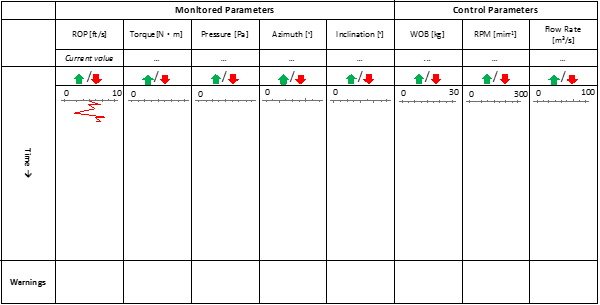
\includegraphics[width=1.0\textwidth]{figures/datadisplay.png}
\caption{Data Display 1}
\label{fig:datadisplay}
\end{figure}

\begin{figure} [H]
\centering
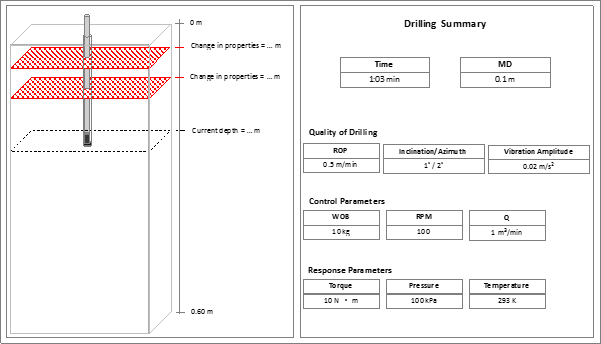
\includegraphics[width=1.0\textwidth]{figures/datadisplay2.png}
\caption{Data Display 2}
\label{fig:datadisplay2}
\end{figure}
